\chapter{(Problem) Analysis}
\begin{itemize}
    \item What is the problem I am looking at?
    \item Analysing papers
    \item What is relevant to include?
    \item Builds on the background chapter
\end{itemize}

In this chapter, we will be doing problem analysis. We will dive deeper into the problem we intend to fix, and we will discuss what the current solutions lack. While the alternatives we present boast about successfull outcomes, there are some shortcomings when comparing them to what we wish to achieve, as well as comparing the respective target audiences. \hfill \\

\section{The problem at hand}

The issue of translating code to some sort of pseudo code has been around for a while (source?), often intended to help people less familiar with code, or perhaps those with no familiarity to code whatsoever, to understand what is being done behind the scenes, and better understanding what product is being built etc. (source??). \hfill \\

We, on the other hand, believe that people who \textit{do} have some familiarity with code could also benefit from being exposed to it. For one, it can be a nice tool for debugging a-little-too-fancy code you did not write yourself, by getting a more abstract view of it. It can also aid beginners in seeing the flow of their code, making them understand how they can improve their code. Unfortunately, there does not seem to be any tools freely available on the market with this target audience in mind: people who also code, but would like to see their code from a different perspective. \hfill \\

Another aspect of pseudo code, is that since it is intended to be a presentation-only tool, you cannot actually verify its semantical properties, that is, if it even does what you want it to do. As Donald Knuth famously put it,

\begin{displayquote}
    I have only proven the algorithm correct, not tested it.\cite{DBLP:books/aw/Knuth68}
\end{displayquote}

Therefore, by manually translating executable code into a non-executable form, we are no longer able to test it, and the work of maintaining both quickly turns into a hassle. We believe that everyone benefits from there persisting a stronger relationship between the original code and the presentation-only pseudocode. \hfill \\

Ever since the concept of pseudocode was introduced, there have been attempts at creating tools to automate the process of translating code to pseudocode. The most noteworthy attempt to deliver pseudocode in text format was presented in a 2015 paper, a tool called Pseudogen. When it comes to translating code to flow charts, we decided to look at Code2Flow, which is widely used in practice today, even in PIT, the Norwegian police's IT service. \hfill \\

\section{Translating code to natural language: Pseudogen}

Pseudogen boasts about generating pseudocode from Python. What the examples in the 2015 paper, as well as a video on their website\footnote{https://ahclab.naist.jp/pseudogen/} show, is rather a line-for-line translation to English. This could be desired in cases where the business people on the team are particularly curious about what the product is really doing under the hood (and the boss cannot afford Cobol developers). Since Pseudogen will translate each line in a slave-like manner, we also translate all error handling. For example, the following two lines

\begin{verbatim}
    except ValueError as e:
        print(e)
\end{verbatim}

will translate to

\begin{verbatim}
    # If ValueError, renamed to e, exception is caught.
        # Call the function print with an argument e
\end{verbatim}

One can speculate as to whether or not anyone gained much knowledge from that, though that is, luckily, not our task. We can also assume the business people would not be overly interested in each single piece of error handling anyway, but the absence of possibility for abstraction can make the translated transcript overwhelmingly verbose. \hfill \\

Due to every line being translated, succinct and elegant list comprehension like

\begin{verbatim}
    a = [f(n) for n in range(-10, 10)]
\end{verbatim}

is translated into this long, tangled spaghetti of words

\begin{verbatim}
    # Call the function f with an argument n for every n in
      range of integers from range 10 negative integer 10,
      substitute the result for a
\end{verbatim}

The target audience is people who prefer the English translation to the Python code. The two examples we just provided show that the target audience is unlikely to be someone who has any background with at least programming or mathematics, which is in turn the target audience for \textit{our} tool. \hfill \\

The choice of creating a tool like Psuedogen for a programming language like Python makes sense as a prototype, because Python is already so closely related to ``natural language''. Using syntax like $and$, $or$, colons etc. often makes Python code very easy to read. Thus, imagine a scenario where we declare a list of 10 integers, create a new list by filtering out the even ones, and print the result. In Python, we could do something like

\begin{verbatim}
    numbers = [1, 2, 3, 4, 5, 6, 7, 8, 9, 10]

    even_numbers = [num for num in numbers if num % 2 == 0]

    print("Even numbers:", even_numbers)
\end{verbatim}

This is already so close to what we would have if we were to write the commands in English, making the task of translation simple. Though it makes you wonder, what is even the point of translating that? As we saw earlier, particularly translation of list comprehensions turn out rather messy compared to their succinct Python counterparts. Another argument against its usefullness is that the listing above is a fully fledged program, ready to be interpreted! If a user is still unsure about what the program is doing, executing it will certainly silence their doubts. \hfill \\

Now, let us analyse the same program written in the Go programming language:

\begin{verbatim}
    numbers := []int{1, 2, 3, 4, 5, 6, 7, 8, 9, 10}

    var evenNumbers []int

    for _, num := range numbers {
        if num % 2 == 0 {
            evenNumbers = append(evenNumbers, num)
        }
    }

    fmt.Println("Even numbers:", evenNumbers)
\end{verbatim}

This program is objectively much less decipherable than its Python counterpart. For starters, it is properties of being statically typed introduces patterns like $[]int\{\}$ and keywords like $var$. Since we do not have list comprehension, we are forced to iterate the ``numbers''-list with a for-loop. ``range mubers'' yields two values for each instance, the current index and the current value. On top of this, a syntactically correct Go program would require this being inside a function, a main function, and boilerplate code like declaring the package and imports like ``fmt''. A translation of the Go program would surely be more desired than a translation of the Python program. Sadly, Pseudogen does not offer this. \hfill \\

It also makes you think, did William Shakespeare really write his entire collection of works in pseudocode?

\section{Psnodig vs. Pseudogen}

Let us take a more thorough look at Pseudogen, and how it differs to Psnodig. Their transpiler is currently designed to work with a subset of the Python programming language\footnote{https://www.python.org/}. The output target is pure natural language, precisely what you are reading now. \hfill \\

Despite being a programming language notoriously known for using plain English where many other programming languages use more technical notation ($and$ instead of $\&\&$, $or$ instead of $||$ etc.), Python still bears the mark of being a programming language. People not familiar with programming and/or mathematics might struggle to understand what the \% (modulo) is and what it is for. \hfill \\

That is where Pseudogen comes in. Not only is mathematical notation like

\begin{displayquote}
    if n \% 3 == 0:
\end{displayquote}

transpiled to

\begin{displayquote}
    if n is divisible by 3,
\end{displayquote}

but also programming language specific elements like

\begin{displayquote}
    raise TypeError('n is not an integer')
\end{displayquote}

is transpiled to

\begin{displayquote}
    throw a TypeError exception with a message ...
\end{displayquote}

\begin{figure}[ht]
    \centering
    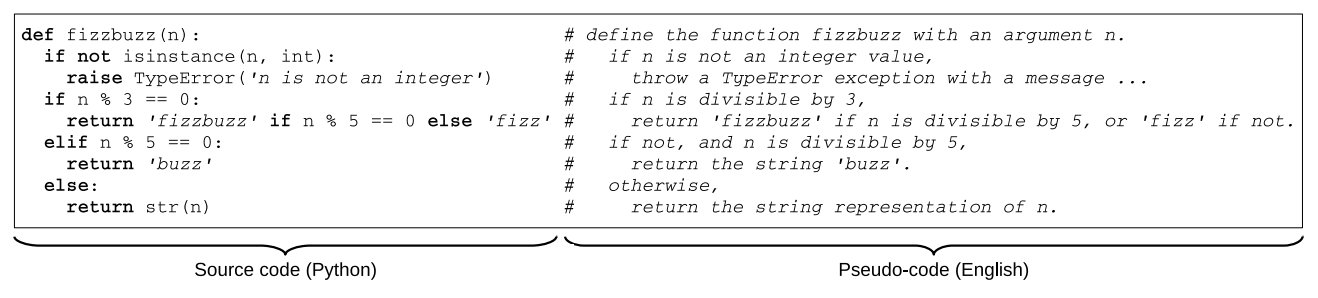
\includegraphics[scale=0.52]{assets/odaetal.png}
    \caption{Example of source code written in Python and corresponding pseudo-code written in English from Oda et. al}
    \label{fig:enter-label}
\end{figure}

For an audience with little to no programming language expereince, this is likely fine. A boss that wishes to see what her engineers are spending their time on, a curious George wanting to get insight into TikToks algorithms, and anyone in between. \hfill \\

Psnodig, however, offers pseudocode for a different crowd: people, primarily the ones involved in academia, who already have some experience with writing and reading code. If you know that the \% symbol stands for modulo, and that it represents the action of returning the remainder of a division operation, it is no longer benefitial to constantly read the verbose description. When reading a novel in italian after successfully learning the language, you would likely prefer each page driving the story forward, rather than having an english word-for-word translation on every other page. \hfill \\

While Pseudogen drives the abstraction levels of Python down to natural language, Psnodig instead wishes to stay closer to the code, while still allowing for an extra layer of abstraction when the implementation is clumsy or too language-specific.

\section{Translating code to flowcharts: Code2Flow}

also say what is wrong about the flowcharts, show examples of code etc. maybe inconsistencies?

\section{Psnodig vs. Code2Flow}

Let us take a more thorough look at Code2Flow, and how it differs to Psnodig. Code2Flow lets the user create flowcharts with natural language, decorated with a C-like syntax.

It mainly consists of

\begin{itemize}
    \item start- and end expressions, drawn as red ovals
    \item other expressions, drawn as blue rectangles
    \item conditionals, loops and match statements, drawn as red red rhombuses
    \item comments, drawn as orange rectangles
\end{itemize}

Expressions are separated by semicolons. This is the default colour scheme, though there are also three others the user can pick.

\begin{figure}[ht]
    \centering
    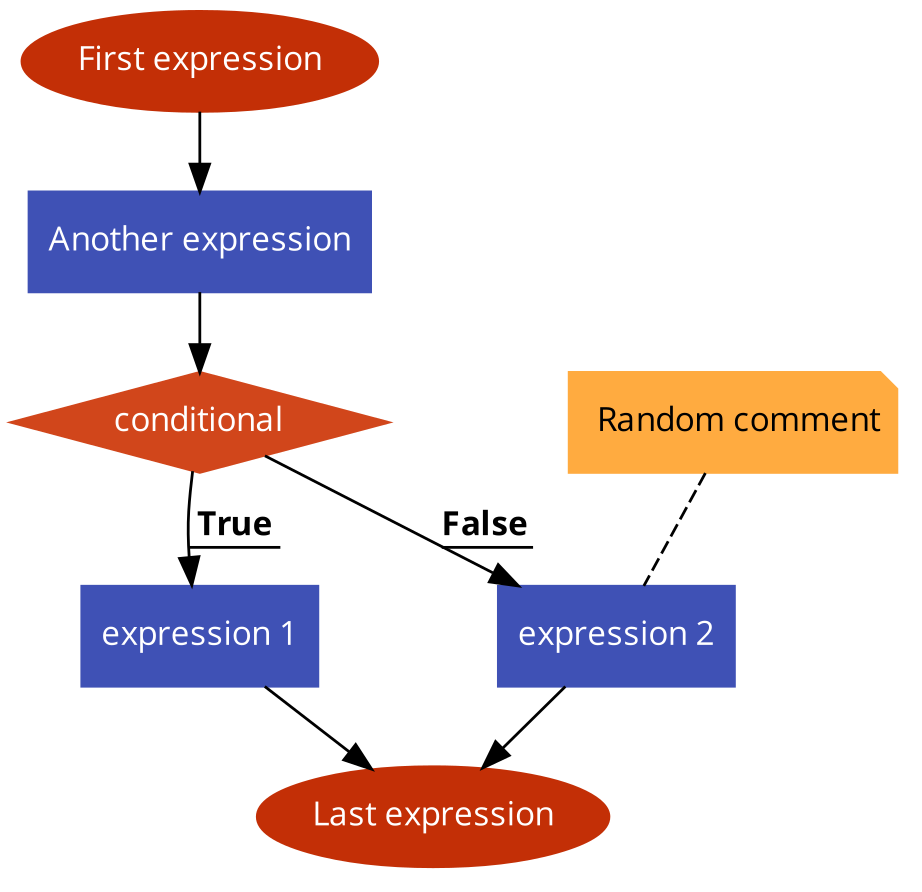
\includegraphics[scale=0.2]{assets/code2flow_example.png}
    \caption{Example of a program written with Code2Flow}
    \label{fig:enter-label}
\end{figure}

The above diagram is the result of writing the following code in the online code2flow interpreter:

\begin{lstlisting}
    First expression;
    Another expression;
    if (conditional) {
      expression 1;
    } else {
      expression 2; // Random comment
    }
    Last expression;
\end{lstlisting}

Using flowcharts to visualise a program is nothing new, however again we have a situation where the autor has to re-write their algorithm in yet \textit{another} language, and hope they did not drift too far from their original code. Naturally, these flowcharts cannot be tested with any input, and are meant to be presentation-only. \hfill \\

Psnodig, on the other hand, makes a point of transpiling syntax-error-free code, which the author can first test on whatever input they want. First then are they allowed to transpile their code, which does not require them to write anything again, unless they want to tweak any details.